\documentclass[12pt]{article}
\usepackage[utf8]{inputenc}
\usepackage[english]{babel}
\usepackage{geometry}
\usepackage{graphicx}
\usepackage{amsmath}
\usepackage{array}
\usepackage{hyperref}
\usepackage{fancyhdr}
\usepackage{lipsum} 
\usepackage{subfig}
\usepackage{float}
\usepackage{booktabs} 
\usepackage{hyperref}
\usepackage{array} 
\usepackage[table]{xcolor}
\usepackage{makecell}
\usepackage{tabularx}
\usepackage{float}
\usepackage{tikz}
\usetikzlibrary{positioning, shapes, arrows}

\geometry{a4paper, margin=1in}
\hypersetup{
    colorlinks=true,
    linkcolor=blue,
    filecolor=magenta,      
    urlcolor=cyan,
}

\begin{document}

\begin{titlepage}
    \begin{center}
        \vspace*{2.2cm}
        
        \Huge
        \textbf{Hitzontzi : Euskera Transcription}

        \vspace{1.75cm}

        
\includegraphics[width=0.6\textwidth]{Hitzontzi.png} 
        \vspace{1.75cm} % adjust vertical space after image

        \Large
        Karim Abu-Shams\\
        \vspace{0.2cm}
        Iker Urdiroz Arroyo\\

        \vspace{1.8cm}

        \huge
        Master in Machine Learning - UPNA\\
        
    \end{center}
\end{titlepage}


\tableofcontents
\newpage


\section{Introduction}

The rise of large-scale foundation models, such as OpenAI's Whisper, has revolutionized the field of Automatic Speech Recognition (ASR), achieving performance levels comparable to human transcription in high-resource languages like English and Spanish \cite{radford2022whisper}. However, these multilingual architectures often face significant limitations when applied to minority or low-resource languages such as Euskera. Due to "capacity dilution," these models prioritize dominant languages, leading to suboptimal accuracy and higher error rates for Basque speakers \cite{bapna2022mslam}.

Furthermore, the computational demands of these heavy architectures often necessitate cloud-based processing, which introduces concerns regarding user privacy, latency, and the requirement for constant internet connectivity. While lightweight alternatives exist, they frequently yield unacceptable Word Error Rates (WER) for morphologically complex languages like Basque, where metrics such as Character Error Rate (CER) often provide a more accurate reflection of linguistic capture \cite{acl2024complexity}.

This project addresses the accuracy-efficiency trade-off by developing a high-performance, privacy-preserving ASR system for Euskera designed to run entirely on-device. By leveraging a composite dataset of approximately 896 hours—combining sources such as Mozilla’s Common Voice, the Basque Parliament Speech Corpus \cite{mdpi2024basque}, and OpenSLR 76, we aim to capture a wide range of acoustic environments and formal discourse.

The technical core of this work involves a complex pipeline of:
\begin{itemize}
    \item \textbf{Fine-tuning:} Adapting pre-trained models to specific Basque dialects and accents.
    \item \textbf{Model Compression:} Utilizing techniques such as Int8 Quantization and Pruning to fit model constraints onto mobile and consumer hardware without significant performance loss.
\end{itemize}

Beyond technical optimization, this project serves a critical social purpose by contributing to the "digital survival" of the Euskera community \cite{hernaez2022ele}. By lowering the hardware barriers to high-quality ASR, we provide a scalable, offline-first solution that eliminates recurring cloud costs and ensures data sovereignty for journalists, administrators, and language learners alike.

\subsection{Problem Statement and Impact}
The core problem this project addresses is the accuracy-efficiency trade-off in Automatic Speech Recognition (ASR) for minority languages. Speech-driven edge devices face a fundamental trade-off between cloud-based solutions, which offer stronger language understanding capabilities at the cost of latency, connectivity dependence, and privacy concerns, and edge-based solutions, which provide low latency and improved privacy but are constrained by limited computational resources \cite{asta2025}. Current solutions often force users to rely on lightweight models that produce unacceptable Word Error Rates (WER) for morphologically complex languages, where traditional metrics like WER often fail to accurately reflect linguistic performance \cite{cer2025}. 

Deploying a high-accuracy, privacy-preserving, and entirely on-device ASR system contributes to the digital survival and democratization of AI for the Euskera community. Furthermore, an offline-first approach eliminates recurring cloud inference costs, providing significant operational value.

\subsection{Target Audience and Stakeholders}
The primary beneficiaries of this solution include:
\begin{itemize}
    \item \textbf{Basque Speakers and Learners:} Individuals who require real-time transcription for accessibility, productivity, or language learning without relying on data connectivity. On-device ASR systems prioritize data privacy and security by eliminating the need for Internet connectivity or external processing \cite{ieee2025}.
    \item \textbf{Journalists and Administration:} Professionals handling sensitive interviews or official meetings where data privacy is an absolute requirement, benefiting from models executed locally without communicating with external servers \cite{mdpi2024}.
    \item \textbf{Technological Ecosystem:} Software developers seeking open-source reference implementations for deploying Transformer-based audio models on mobile and edge architectures.
\end{itemize}

\subsection{Business and Machine Learning Objectives}
This project balances strict linguistic accuracy with operational and business viability through a three-tiered objective system:

\subsubsection{Machine Learning Objectives}
\begin{itemize}
    \item \textbf{Optimize Linguistic Quality:} The primary metric is the Character Error Rate (CER). As ASR systems expand to multilingual contexts, WER fails in various ways, particularly with morphologically complex languages or those without clear word boundaries \cite{cer2025}. CER avoids many of these challenges, exhibits greater consistency across writing systems, and correlates more closely with human judgments of transcription quality \cite{cer2025}.
    \item \textbf{Maintain Baseline Intelligibility:} Ensure that transcription accuracy remains functionally equivalent to the full-precision baseline after model compression (such as Int8 Quantization).
\end{itemize}

\subsubsection{Business and Operational Objectives}
\begin{itemize}
    \item \textbf{Ensure On-Device Viability:} Achieve a Real-Time Factor (RTF) of less than 1.0 on CPU inference, minimizing latency while maintaining high accuracy, which is essential for real-time voice applications \cite{ieee2025}.
    \item \textbf{Low Latency Interaction:} Attain a Time To First Token (TTFT) enough to guarantee immediate feedback and avoid the sensation of system unresponsiveness.
    \item \textbf{Minimize User Effort:} Maintain a Human Correction Rate (HCR) below 0.15, meaning less than 15\% of the generated characters require manual editing by the user.
    \item \textbf{Cost Efficiency:} Deliver a "deploy-once" mobile artifact that provides a scalable solution with zero marginal cost per transcription.
\end{itemize}




\section{Deployment and Monitoring}

The deployment logic of \textit{Hitzontzi} revolves around a containerized, local-first architecture that prioritizes privacy, ease of use, and flexibility across hardware configurations (CPU vs. GPU). The overarching design separates the frontend client from the transcription backend, allowing them to scale or be updated independently while running within the same isolated environment.

\subsection{Serving Infrastructure}
The serving infrastructure relies on a lightweight, modular stack designed for seamless local hosting:
\begin{itemize}
    \item \textbf{API (FastAPI):} The core backend is implemented in Python using FastAPI. It exposes a REST endpoint (\texttt{/transcribe}) for handling standalone audio file uploads, and a WebSocket endpoint (\texttt{/ws/transcribe}) for streaming real-time audio chunks. FastAPI guarantees high concurrency and fast routing with minimal overhead.
    \item \textbf{Containerization (Docker):} The entire application is packaged using Docker. We maintain two primary distribution strategies:
    \begin{itemize}
        \item \textit{Slim:} The model weights are mounted dynamically from the host file system. This keeps the Docker image lightweight ($\sim$1 GB) and speeds up the build process during development.
        \item \textit{Bundled:} The fine-tuned Whisper model is baked directly into the Docker image ($\ge$ 2 GB). This provides a completely self-contained, "plug-and-play" artifact that can run on any machine without requiring the user to download model weights separately.
    \end{itemize}
    \item \textbf{Hosting:} The system is designed to run locally (via \texttt{localhost}) managed by \texttt{docker-compose}. Hardware acceleration is natively supported through specific profiles (e.g., \texttt{whisper-gpu-bundled}) leveraging the NVIDIA Container Toolkit.
\end{itemize}

\subsection{Architecture Diagram}
The following diagram illustrates the data flow from user input down to the transcription output. The user interacts entirely with a vanilla HTML/JS frontend, which captures microphone data or file uploads, passing them to the FastAPI backend. The audio is decoded via FFmpeg and processed by the in-memory Hugging Face Pipeline, returning the transcribed text.

\begin{figure}[H]
    \centering
    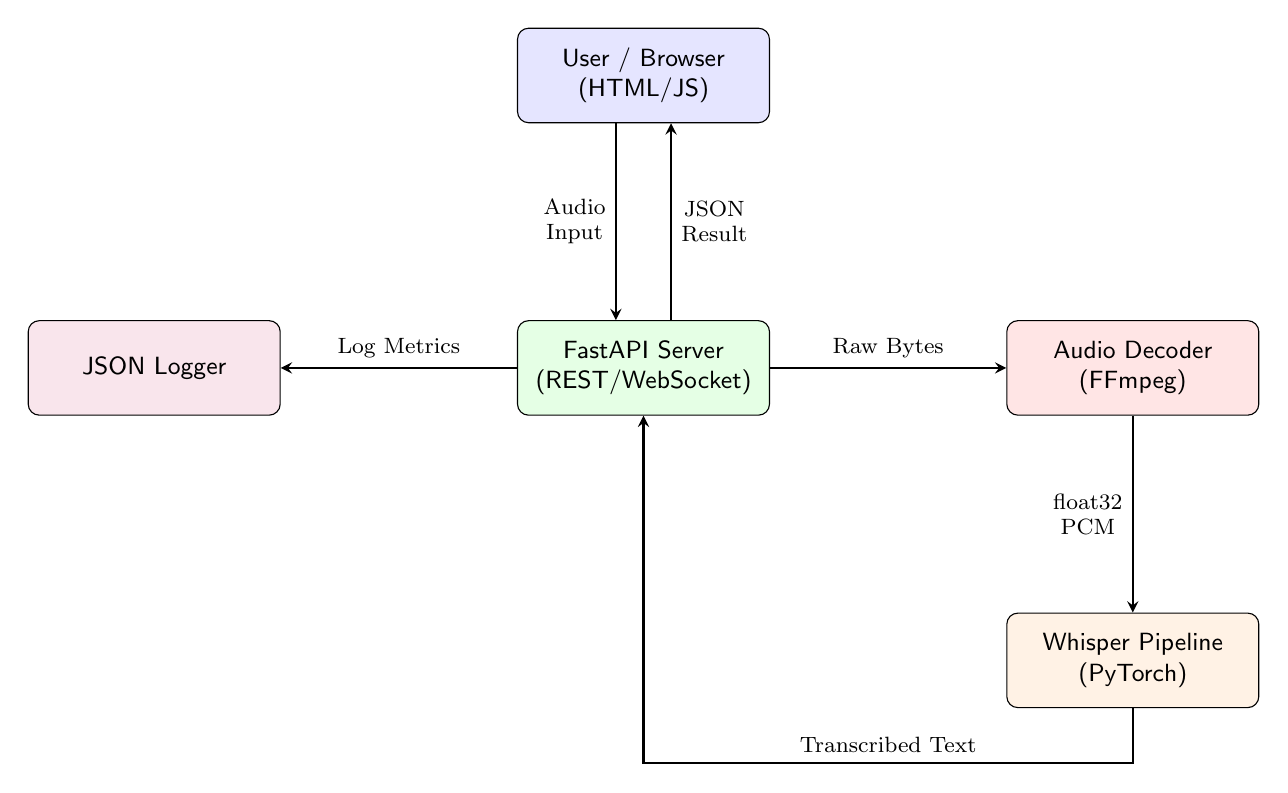
\begin{tikzpicture}[
        node distance=2.5cm and 3cm,
        box/.style={draw, rectangle, rounded corners, align=center, minimum width=3.2cm, minimum height=1.2cm, font=\sffamily\small},
        arrow/.style={-stealth, thick, align=center}
    ]
        % Nodes
        \node[box, fill=blue!10] (user) {User / Browser\\(HTML/JS)};
        \node[box, fill=green!10, below=of user] (api) {FastAPI Server\\(REST/WebSocket)};
        \node[box, fill=purple!10, left=of api] (logger) {JSON Logger};
        \node[box, fill=red!10, right=of api] (ffmpeg) {Audio Decoder\\(FFmpeg)};
        \node[box, fill=orange!10, below=of ffmpeg] (model) {Whisper Pipeline\\(PyTorch)};
        
        % Arrows
        % Between User and API
        \draw[arrow] (user.240) -- node[left]{\footnotesize Audio\\[-1mm]\footnotesize Input} (api.120);
        \draw[arrow] (api.60) -- node[right]{\footnotesize JSON\\[-1mm]\footnotesize Result} (user.300);
        
        % Between API and FFmpeg
        \draw[arrow] (api.east) -- node[above]{\footnotesize Raw Bytes} (ffmpeg.west);
        
        % Between FFmpeg and Model
        \draw[arrow] (ffmpeg.south) -- node[left]{\footnotesize float32\\[-1mm]\footnotesize PCM} (model.north);
        
        % Return from Model to API
        \draw[arrow] (model.south) -- +(0,-0.7) -| node[above, pos=0.25]{\footnotesize Transcribed Text} (api.south);
        
        % Logger
        \draw[arrow] (api.west) -- node[above]{\footnotesize Log Metrics} (logger.east);
    \end{tikzpicture}
    \caption{System Architecture Diagram}
    \label{fig:architecture}
\end{figure}

\subsection{Monitoring Strategy}
Although deployed locally, internal observability is critical for profiling performance across varied consumer hardware. The backend incorporates a bespoke logging module that records transcription metrics into a persistent \texttt{JSON} file. The key signals tracked include:
\begin{itemize}
    \item \textbf{Real-Time Factor (RTF) and Elapsed Time:} The ratio of processing time to audio duration. Tracking RTF is vital to ensure the hardware is transcribing faster than the speaker talks (RTF $< 1.0$), which is a hard requirement for the WebSocket real-time mode.
    \item \textbf{Device Utilization (CPU vs. CUDA):} Validates that the application correctly acquired GPU acceleration if requested, preventing silent fallbacks to CPU that would severely degrade performance.
    \item \textbf{Audio Input Levels (RMS):} Tracks the average signal energy. Recording silent or excessively quiet chunks is a common source of model "hallucinations." Monitoring this allows us to diagnose if bad transcriptions are due to microphone misconfigurations.
    \item \textbf{Throughput Metrics (Audio Length, Text Length):} We log the duration of the audio processed alongside the number of generated characters and words. This helps identify edge cases where the model enters a hallucination loop (producing massive text outputs for short audio segments) or fails to output any text.
\end{itemize}

Looking forward, the structured nature of these \texttt{JSON} logs serves as the foundational data layer for an advanced observability pipeline. In future iterations, these logs will be aggregated and ingested into visualization platforms such as \textbf{Grafana}. By doing so, we aim to establish a comprehensive real-time monitoring dashboard capable of visualizing latency distributions across different hardware configurations, configuring automated alerts for sustained high-latency or audio dropout events, and seamlessly tracking the empirical performance of subsequent model deployments.

\section{Conclusions}

The project successfully met its primary Machine Learning objectives, achieving a substantial transcription quality improvement for Euskera compared to the official OpenAI Whisper models. Notably, our fine-tuned Base model exhibited remarkable gains, completely surpassing the baseline performance for this specific language. Regarding operational metrics, inference speed varied significantly depending on the hardware. When leveraging GPU acceleration (CUDA), the model effortlessly achieves Real-Time Factors (RTF) well below 1.0, enabling seamless live transcription. CPU execution, while slower, remains highly viable for asynchronous file processing.

However, the initial business objective of deploying a fully native mobile application was not entirely met. The stringent memory and performance constraints of consumer mobile devices made direct on-device execution challenging without severe performance degradation. To circumvent this, we pivoted towards a highly portable Dockerized architecture. This approach guarantees that the system can be deployed on any standard computer—operating identically across Windows, macOS, or Linux—while still providing extreme ease of use and preserving strict data privacy by running entirely offline. Methodologically, pivoting from a native mobile app to a locally-hosted containerized web application was a crucial lesson in agile workflow, ensuring that the core value proposition was delivered despite smartphone hardware limitations.

Technically, we learned that while fine-tuning acoustic models yields massive accuracy improvements for minority languages, the subsequent deployment pipeline is equally challenging. The trade-off between model precision and edge-device viability requires rigorous evaluation. Given more time and computational resources, we would have heavily invested in advanced model compression and quantization techniques, which would have likely bridged the gap required to successfully execute the model natively on mobile devices. Furthermore, we would have dedicated significant effort to improving the model's lexical punctuation. Currently, the system occasionally struggles with correct comma placement and sentence casing during long, continuous speeches, which remains its weakest point.

\subsection{Future Work}
To guarantee the long-term maintainability and continuous improvement of \textit{Hitzontzi}, future work should focus on addressing the current architectural shortcomings:
\begin{itemize}
    \item \textbf{Dataset Augmentation:} Curate and integrate datasets specifically rich in high-quality punctuation and diverse conversational casing to address current punctuation deficiencies.
    \item \textbf{Orthographic Correction Layer:} Implement a lightweight post-processing spell checker or language model to automatically refine and correct the minor morphological errors the acoustic model still produces.
    \item \textbf{Real-World Monitoring:} Operationalize the currently implemented \texttt{JSON} logging system to build a comprehensive monitoring dashboard (e.g., using Grafana). This will allow us to study the primary failure modes, track hallucination rates, and seamlessly understand how the model behaves across real-world environments.
\end{itemize}


\begin{thebibliography}{99}

% Referencia oficial del modelo Whisper de OpenAI
\bibitem{radford2022whisper} 
A. Radford \textit{et al.}, ``Robust speech recognition via large-scale weak supervision,'' \textit{arXiv preprint arXiv:2212.04356}, 2022.

% Referencia sobre el problema de "capacity dilution" en modelos multilingües (mSLAM)
\bibitem{bapna2022mslam}
A. Bapna \textit{et al.}, ``mSLAM: Massively multilingual joint pre-training for speech and text,'' \textit{arXiv preprint}, 2022.

% Referencia sobre la complejidad morfológica/ortográfica y su impacto en el ASR (WER vs CER)
\bibitem{acl2024complexity}
``Language Complexity and Speech Recognition Accuracy: Orthographic Complexity Hurts, Phonological Complexity Doesn't,'' \textit{Proceedings of the Association for Computational Linguistics (ACL)}, 2024.

% Referencia oficial sobre el corpus del Parlamento Vasco y desarrollo de ASR
\bibitem{mdpi2024basque}
``A Bilingual Basque–Spanish Dataset of Parliamentary Sessions for the Development and Evaluation of Speech Technology,'' \textit{MDPI Applied Sciences}, vol. 14, no. 5, p. 1951, 2024.

% Referencia del proyecto European Language Equality (ELE) específico para el euskera
\bibitem{hernaez2022ele}
I. Hernáez, E. Navas, I. Odriozola, K. Sarasola, and A. Diaz de Ilarraza, ``Language Report Basque,'' in \textit{European Language Equality}, 2022, pp. 95--98.

\bibitem{asta2025}
``Adaptive Edge-Cloud Inference for Speech-to-Action Systems Using ASR and Large Language Models,'' \textit{arXiv preprint arXiv:2512.12769}, 2025.

\bibitem{cer2025}
``Advocating Character Error Rate for Multilingual ASR Evaluation,'' \textit{ResearchGate}, 2025.

\bibitem{ieee2025}
``On-Device Automatic Speech Recognition for Low-Resource Languages in Mixed Reality Industrial Metaverse Applications,'' \textit{IEEE}, 2025.

\bibitem{mdpi2024}
``On-Device Automatic Speech Recognition for IIoT and Extended Reality Industrial Metaverse Applications,'' \textit{MDPI}, 2024.

\end{thebibliography}
\end{document}